%\documentclass[aspectratio=169]{beamer} %1920x1080 resolution
\documentclass[handout, aspectratio=169]{beamer}
\usepackage{../../../LatexTemplatesAndSamples/mastering_ir_derivatives_beamer} % My custom style

% This goes together with handout feature above
%\pgfpagesuselayout{2 on 1}[border shrink=2mm]

% Needs to be set for each class
\subtitle{Introduction to Building of Interest Rate Curves}

\begin{document} 

\input{../../../LatexTemplatesAndSamples/firstThreeSlides.tex}

\section{Overview, Purpose and Concept of Building Curves}
 
\begin{frame}{Purpose of Building Curves}
	\begin{itemize}
		\item \textbf{"Everything starts with interest rate curves"} - Interest rate curves serve as the foundation for various financial analyses and applications
		\item Valuing any financial instrument depends on interest rates, which can be extracted or implied from these curves
	\end{itemize}
\end{frame}

\begin{frame}{Concept of Building Curves - 1}
	\begin{itemize}
		\item Objective: Develop a rational approach to estimate fair interest rates
		\item Considerations:
		\begin{itemize}
			\item Interest rates vary with the term of the instrument and include a risk premium
			\item Arbitrage opportunities should be avoided
		\end{itemize}
		\item Approach to build curve: 
		\begin{itemize}
			\item Utilize widely used instruments to estimate rates
			\item Find rates to price all instruments to market
		\end{itemize}
		\item Representation of built curve
		\begin{itemize}
			\item Curves are stored as a term structure of zero rates
		\end{itemize}
	\end{itemize}
\end{frame}

\begin{frame}{Concept of Building Curves - 2}
	\begin{itemize}
		\footnotesize
		\item The curves we estimate represent the interest rates at which investors actually trade, rather than the expected rates
		\item The forward rate differs from the expected spot rate due to the inclusion of a risk premium
	\end{itemize}
	\onslide<3->{
		\begin{figure}
			\centering
			\includegraphics[width=0.5\linewidth]{Expected short rate vs realized short rate TGIR.png}
			\caption{Term Structure of Rates Compared to the Realized Short-term Spot Rate}
		\end{figure} 
	}
\end{frame}

\section{Simplified Example of Building Curves using Discount Bonds}

\begin{frame}{Simplified: Use Discount Bond - 1}
	\begin{itemize}
		\small
		\item Assume we have 5 bonds maturing over the next 5 years
		\item They are zero coupon bonds with known prices
		\item For illustrative purposes, as these bonds are not liquid in reality
	\end{itemize}
	\onslide<4->{
		\begin{table}[h]
			\centering
			\begin{tabular}{|c|c|c|} 
					\hline
					\textbf{Maturity} & \textbf{\# Days} & \textbf{Price}\\				
						\hline
						1 year & 365 & 98.81 \\ 
						23 months & 700 & 97.35 \\ 
						3 years & 1,095 & 95.03 \\ 
						49 months & 1,490 & 92.54 \\ 
						5 years & 1,825 & 90.48 \\ 
						\hline
			\end{tabular}
			\caption{5 Bonds}
		\end{table}
	}
\end{frame}

\begin{frame}{Simplified: Use Discount Bond - 2}
	\begin{itemize}
		\item To determine today's price, we need to discount the par value of the bond from its maturity value; otherwise, an arbitrage opportunity would arise
		\item We can calculate each zero rate by utilizing a closed-form formula based on this concept
		\item Let $d_i$ represent the number of days between the maturity date of bond $i$ and today
		\item The price $P_i$ of bond $i$ is given by $P_i = DF_{d_i} * \$100$
		\item The discount factor $DF_{d_i}$ is calculated as $DF_{d_i} = e^{-z_{d_i} * d_i / 365}$
		\item Now, solving for $z_{d_i}$ for each bond's maturity allows us to obtain the corresponding zero rates. As an exercise, you can derive the explicit formula for $z_{d_i}$
	\end{itemize}
\end{frame}

\begin{frame}{Simplified: Use Discount Bond - 3}
	\begin{itemize}
		\item After deriving zero rates, we have the following bond data:
	\end{itemize}
	\begin{table}[h]
		\centering
   		\begin{tabular}{|c|c|c|c|} 
	 		\hline
	 		\textbf{Maturity} & \textbf{\# Days}  & \textbf{Price} & \textbf{Zero Rate}\\				
	 			\hline
	 			1 year & 365 & 98.81 & 1.2\% \\ 
	 			23 months & 700 & 97.35 & 1.4\% \\ 
	 			3 years & 1,095 & 95.03 & 1.7\% \\ 
	 			49 months & 1,490 & 92.54 & 1.9\% \\ 
	 			5 years & 1,825 & 90.48 & 2\% \\ 
	 			\hline
   		\end{tabular}
	   \caption{Bond Information including Zero Rates}
	\end{table}
\end{frame}


\begin{frame}{Simplified: Use Discount Bond - 4}
	\begin{itemize}
		\item Let's graph our first zero curve based on our simplified assumptions
	\end{itemize}
	\begin{adjustbox}{max height=0.7\textheight}
		\centering
	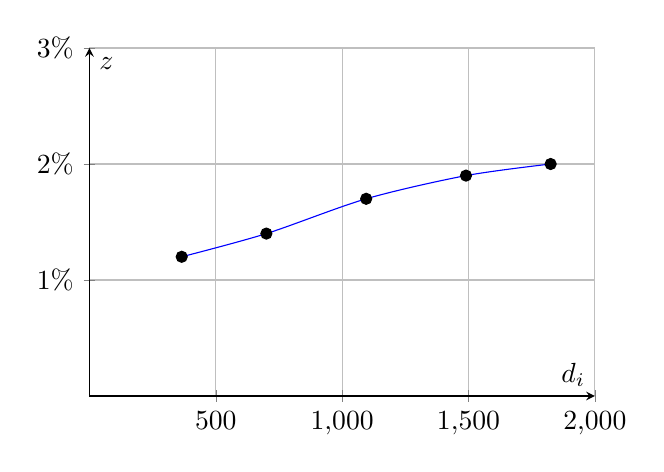
\begin{tikzpicture}
		\centering
		\begin{axis}[
			axis lines=middle,
			xlabel=$d_i$,
			ylabel=$z$,
			xmin=0, xmax=2000,
			ymin=0, ymax=0.03,
			% xtick={1,2,3,4},
			ytick={0.01,0.02,0.03,0.04},
			% xticklabels={1,2,3,4},
			yticklabel={\pgfmathparse{100*\tick}\pgfmathprintnumber{\pgfmathresult}\%},
			width=8cm,
			height=6cm,
			grid=both,
			grid style={gray!50},
			scaled ticks=false %remove scientific notation
			]
		  
		  \addplot[only marks, mark=*] coordinates {
			(365, 0.012)
			(700, 0.014)
			(1095, 0.017)
			(1490, 0.019)
			(1825, 0.02)
		  };
		  
		  \addplot[smooth,blue] coordinates {
			(365, 0.012)
			(700, 0.014)
			(1095, 0.017)
			(1490, 0.019)
			(1825, 0.02)
		  };
		  \end{axis}
		\end{tikzpicture}
	\end{adjustbox}
\end{frame}

\section{Building Curves using Money Market Rates, Futures and Swaps}
\subsection{Introduction to the Structure of the Curve and its Segments}
\begin{frame}{Introduction to the Structure of the Curve and its Segments}
  	\begin{itemize}	
		\item USD/LIBOR illustration to build curve \footnote{\tiny LIBOR ceased to exist mid-2023 but still very good for illustration}
		\item Deriving a zero curve from liquid instruments
		\item Conceptually good points, although slightly different instruments were used in practice
	\end{itemize}
	\onslide<4->{
		\begin{table}[t]
			\centering
			\begin{adjustbox}{max width=\textwidth, max height=0.25\textheight}
				\begin{tabular}{|c|c|c|} 
					\hline
					\multicolumn{3}{|c|}{\textbf{Market Data as of 29-Jan-2019}} \\
					\hline
					\textbf{Type} & \textbf{Date}  & \textbf{Rate}\\				
					\hline
					MM & 2D & 4.875\% \\
					MM & 1M & 4.875\% \\
					MM & 3M & 4.9\% \\
					\hline
					FUT & MAR-19 & 95.06 \\
					FUT & JUN-19 & 95.12 \\
					... & ... & \\
					\hline
					SWAP & 2Y & 5.125\% \\
					SWAP & 3Y & 5.178\% \\
					... & ... & \\
					\hline
				\end{tabular}
			\end{adjustbox}
		\end{table}
	}
\end{frame}

\subsection{Money Markets}
\begin{frame}{Derive the First Zero Rate for 2D Money Market Point}
  	\begin{columns}[T]
	  \begin{column}{0.4\textwidth}
		  \begin{table}[t]
			  \centering
			  \begin{adjustbox}{max width=\textwidth, max height=\textheight}
				  \begin{tabular}{|c|c|c|c|} 
					  \hline
					  \multicolumn{4}{|c|}{\textbf{Market Data as of 29-Jan-2019}} \\
					  \hline
					  \textbf{Type} & \textbf{Date}  & \textbf{Rate} & \textbf{Zero}\\				
					  \hline
					  MM & 2D & 4.875\% &\\
					  MM & 1M & 4.875\% &\\
					  MM & 3M & 4.9\% &\\
					  \hline
					  FUT & MAR-19 & 95.06 &\\
					  FUT & JUN-19 & 95.12 &\\
					  ... & ... & &\\
					  \hline
					  SWAP & 2Y & 5.125\% &\\
					  SWAP & 3Y & 5.178\% &\\
					  ... & ... & &\\
					  \hline
				  \end{tabular}
			  \end{adjustbox}
		  \end{table}
	  \end{column}
	  
	  % 0.4+0.7 is over 1 but it looks good
	  \begin{column}{0.7\textwidth}
		  \begin{table}[t]
			  \centering
			  \begin{adjustbox}{max width=0.6\textwidth}
				  \begin{tabular}{|c|c|c|} 
					  \hline
					  \multicolumn{3}{|c|}{\textbf{Flows for 2D rate of 4.875\%}} \\
					  \hline
					  \textbf{Date} & \textbf{Amount}  & \textbf{Required NPV}\\				
					  \hline
					  29-Jan-19 & \$100 & \$100 \\
					  \hline
					  31-Jan-19 & -\$100.0271 & -\$100 \\
					  \hline
				  \end{tabular}
			  \end{adjustbox}
		  \end{table}
		  \begin{itemize}
			\item We need to define the discount factor (DF) to make the sum of NPV values \$0
			\item Recall, we have $DF = e^{(-z \cdot \frac{\# \text{ days}}{365})}$
			\item So, $z = \ln(\frac{100.0271}{100}) \cdot \frac{365}{2}$
			\item and, $z = 4.94204\%$
		  \end{itemize}
	   \end{column}
  \end{columns}
\end{frame}

\begin{frame}{Derive the next Zero Rate for 1M Money Market Point}
	\begin{columns}[T]
		\begin{column}{0.4\textwidth}
			\begin{table}[t]
				\centering
				\begin{adjustbox}{max width=\textwidth, max height=\textheight}
					\begin{tabular}{|c|c|c|c|} 
						\hline
						\multicolumn{4}{|c|}{\textbf{Market Data as of 29-Jan-2019}} \\
						\hline
						\textbf{Type} & \textbf{Date}  & \textbf{Rate} & \textbf{Zero}\\				
						\hline
						MM & 2D & 4.875\% & \textbf{4.94204\%} \\
						MM & 1M & 4.875\% &\\
						MM & 3M & 4.9\% &\\
						\hline
						FUT & MAR-19 & 95.06 &\\
						FUT & JUN-19 & 95.12 &\\
						... & ... & &\\
						\hline
						SWAP & 2Y & 5.125\% &\\
						SWAP & 3Y & 5.178\% &\\
						... & ... & &\\
						\hline
					\end{tabular}
				\end{adjustbox}
			\end{table}
		\end{column}
		
		% 0.4+0.7 is over 1 but it looks good
		\begin{column}{0.7\textwidth}
			\begin{table}[t]
				\centering
				\begin{adjustbox}{max width=0.55\textwidth}
					\begin{tabular}{|c|c|c|} 
						\hline
						\multicolumn{3}{|c|}{\textbf{Flows for 1M rate of 4.875\%}} \\
						\hline
						\textbf{Date} & \textbf{Amount}  & \textbf{Required NPV}\\				
						\hline
						31-Jan-19 & \$100 & \$99.9729 \\
						\hline
						28-Feb-19 \footnote{\tiny Rolled date to good business day with Modified Following rolling convention} & -\$100.3792 & -\$99.9729 \\
						\hline
					\end{tabular}
				\end{adjustbox}
			\end{table}
			\begin{itemize}
				\footnotesize
				\item We know the zero rate of 31-Jan-19
				\item Find next $z$ so, $\sum_{i=1}^{n} NPV(Flow_i) = \$0$
				\item Flows are at spot date and 28-Feb-19
				\item We receive \$100 spot and pay back $\$100 \cdot 4.875\% \cdot \frac{28}{360} = \$100.3792$
				\item So, $z = \ln(\frac{100.3792}{99.9729}) \cdot \frac{365}{30}$
				\item and therefore, $z = 4.93394\%$
			\end{itemize}
		 \end{column}
	\end{columns}
\end{frame}

\begin{frame}{Derive the next Zero Rate for 3M Money Market Point}
	\begin{columns}[T]
		\begin{column}{0.4\textwidth}
			\begin{table}[t]
				\centering
				\begin{adjustbox}{max width=\textwidth, max height=\textheight}
					\begin{tabular}{|c|c|c|c|} 
						\hline
						\multicolumn{4}{|c|}{\textbf{Market Data as of 29-Jan-2019}} \\
						\hline
						\textbf{Type} & \textbf{Date}  & \textbf{Rate} & \textbf{Zero}\\				
						\hline
						MM & 2D & 4.875\% & 4.94204\% \\
						MM & 1M & 4.875\% & \textbf{4.93394\%} \\
						MM & 3M & 4.9\% &\\
						\hline
						FUT & MAR-19 & 95.06 &\\
						FUT & JUN-19 & 95.12 &\\
						... & ... & &\\
						\hline
						SWAP & 2Y & 5.125\% &\\
						SWAP & 3Y & 5.178\% &\\
						... & ... & &\\
						\hline
					\end{tabular}
				\end{adjustbox}
			\end{table}
		\end{column}
		
		% 0.4+0.7 is over 1 but it looks good
		\begin{column}{0.7\textwidth}
			\begin{table}[t]
				\centering
				\begin{adjustbox}{max width=0.6\textwidth}
					\begin{tabular}{|c|c|c|} 
						\hline
						\multicolumn{3}{|c|}{\textbf{Flows for 3M rate of 4.9\%}} \\
						\hline
						\textbf{Date} & \textbf{Amount}  & \textbf{Required NPV}\\				
						\hline
						31-Jan-19 & \$100 & \$99.9729 \\
						\hline
						30-Apr-19 & -\$101.2114 & -\$99.9729 \\
						\hline
					\end{tabular}
				\end{adjustbox}
			\end{table}
			\begin{itemize}
				\item We know zero rates up to 28-Feb-19
				\item Find $z$ for 30-Apr-19 so that $\sum_{i=1}^{n} NPV(Flow_i) = \$0$
				\item So, $z = \ln(\frac{101.2114}{99.9729}) \cdot \frac{365}{91}$
				\item and therefore, $z = 4.93829\%$
			\end{itemize}
		 \end{column}
	\end{columns}
\end{frame}

\subsection{Zero Rate Interpolation}
\begin{frame}{Interpolation of Zero Rates}
	\pause
	\begin{itemize}
		\item The zero curve consists of distinct data points
		\item Interpolation is required for values not present on the curve
		\item For the first futures contract, we require $z$ on the starting date
		\item There are many interpolation methods
		\item Smoothing forward rates is common practice
	\end{itemize}
	\begin{block}{Linear interpolation of Zero Rate}
		\small Given, $z_1$ at time $t_1$ and $z_2$ at time $t_2$ interpolate $z$ at time $t$:
		\[
		z = z_1 + (z_2 - z_1) \cdot \frac{t - t_1}{t_2 - t_1} = \frac{z_2 \cdot (t - t_1) + z_1 \cdot (t_2 - t)}{t_2 - t_1}
		\]
	\end{block}
\end{frame}

\subsection{Interest Rate Futures}
\begin{frame}{Derive the next Zero Rate for first Futures contract - 1}
	\begin{itemize}
		\item Eurodollar future represents a 3 month forward rate
		\item Prices are available for up to 3-4 years into the future
		\item It's common to use futures up to 1-2 years
		\item The price of 95.06 implies rate of 4.94\%
		\begin{block}{Futures Price to Rate Conversion}
			\begin{align*}
				Rate & = \frac{100 - Futures\ Price}{100}
			\end{align*}
		\end{block}
		\item The length of the future can be interpreted as 3M or contract to contract 
		\item The start and end dates are determined by exchanges
	\end{itemize}
\end{frame}

\begin{frame}{Derive the next Zero Rate for first Futures contract - 2}
	\begin{columns}[T]
		\begin{column}{0.4\textwidth}
			\begin{table}[t]
				\centering
				\begin{adjustbox}{max width=\textwidth, max height=\textheight}
					\begin{tabular}{|c|c|c|c|} 
						\hline
						\multicolumn{4}{|c|}{\textbf{Market Data as of 29-Jan-2019}} \\
						\hline
						\textbf{Type} & \textbf{Date}  & \textbf{Rate} & \textbf{Zero}\\				
						\hline
						MM & 2D & 4.875\% & 4.94204\% \\
						MM & 1M & 4.875\% & 4.93394\% \\
						MM & 3M & 4.9\% & \textbf{4.93829\%}\\
						\hline
						FUT & MAR-19 & 95.06 &\\
						FUT & JUN-19 & 95.12 &\\
						... & ... & &\\
						\hline
						SWAP & 2Y & 5.125\% &\\
						SWAP & 3Y & 5.178\% &\\
						... & ... & &\\
						\hline
					\end{tabular}
				\end{adjustbox}
			\end{table}
		\end{column}
		
		% 0.4+0.7 is over 1 but it looks good
		\begin{column}{0.7\textwidth}
			\begin{table}[t]
				\centering
				\begin{adjustbox}{max width=0.6\textwidth}
					\begin{tabular}{|c|c|c|} 
						\hline
						\multicolumn{3}{|c|}{\textbf{Flows for MAR-19 contract with price 95.06}} \\
						\hline
						\textbf{Date} & \textbf{Amount}  & \textbf{Required NPV}\\				
						\hline
						20-Mar-19 & \$100 & \$99.3263 \\
						\hline
						19-Jun-19 & -\$101.2487 & -\$99.3263 \\
						\hline
					\end{tabular}
				\end{adjustbox}
			\end{table}
			\begin{itemize}
				\footnotesize
				\item Imply fwd rate: $\frac{100 - 95.06}{100} = 4.94\%$
			 	\item Interpolate $z$ for 20-Mar-19 to get the zero rate on the start date of the future
		 		\item Calculate $t, t_1, t_2$ based on days to today
		 		\item $z = z_1 + (z_2 - z_1) \cdot \frac{20}{59} = 4.93537\%$
		 		\item We can now present value the start flow of the future
		 		\item $NPV = \$100 \cdot e^{-4.93537\% \cdot \frac{50}{365}} = \$99.3263$ 
			\end{itemize}
		 \end{column}
	\end{columns}
\end{frame}

\begin{frame}{Derive the next Zero Rate for first Futures contract - 3}
	\begin{columns}[T]
		\begin{column}{0.4\textwidth}
			\begin{table}[t]
				\centering
				\begin{adjustbox}{max width=\textwidth, max height=\textheight}
					\begin{tabular}{|c|c|c|c|} 
						\hline
						\multicolumn{4}{|c|}{\textbf{Market Data as of 29-Jan-2019}} \\
						\hline
						\textbf{Type} & \textbf{Date}  & \textbf{Rate} & \textbf{Zero}\\				
						\hline
						MM & 2D & 4.875\% & 4.94204\% \\
						MM & 1M & 4.875\% & 4.93394\% \\
						MM & 3M & 4.9\% & \textbf{4.93806\%}\\
						\hline
						FUT & MAR-19 & 95.06 &\\
						FUT & JUN-19 & 95.12 &\\
						... & ... & &\\
						\hline
						SWAP & 2Y & 5.125\% &\\
						SWAP & 3Y & 5.178\% &\\
						... & ... & &\\
						\hline
					\end{tabular}
				\end{adjustbox}
			\end{table}
		\end{column}
		
		% 0.4+0.7 is over 1 but it looks good
		\begin{column}{0.7\textwidth}
			\begin{table}[t]
				\centering
				\begin{adjustbox}{max width=0.6\textwidth}
					\begin{tabular}{|c|c|c|} 
						\hline
						\multicolumn{3}{|c|}{\textbf{Flows for MAR-19 contract with price 95.06}} \\
						\hline
						\textbf{Date} & \textbf{Amount}  & \textbf{Required NPV}\\				
						\hline
						20-Mar-19 & \$100 & \$99.3263 \\
						\hline
						19-Jun-19 & -\$101.2487 & -\$99.3263 \\
						\hline
					\end{tabular}
				\end{adjustbox}
			\end{table}
			\begin{itemize}
				\footnotesize
				\item Calculate 19-Jun-19 flow using standard formula
				\item Basis for interest calculation is A/360 by convention 
				\item $\$100 \cdot (1+4.94\% \cdot \frac{91}{360}) = 100.2487$
				\item Find next $z$ so, $\sum_{i=1}^{n} NPV(Flow_i) = \$0$
				\item So, $z = \ln(\frac{100.2487}{99.3263}) \cdot \frac{365}{141}$
				\item and therefore, $z = 4.96262\%$
			\end{itemize}
		 \end{column}
	\end{columns}
\end{frame}

\begin{frame}{Recap and Graph Zero Rates}
	\begin{figure}
		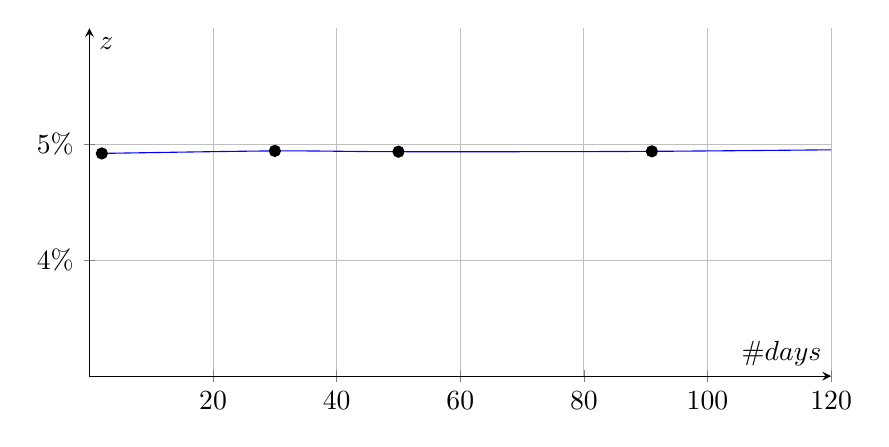
\begin{tikzpicture}
			\begin{axis}[
				axis lines=middle,
				xlabel=$\# days$,
				ylabel=$z$,
				xmin=0, xmax=120,
				ymin=0.03, ymax=0.06,
				% xtick={1,2,3,4},
				ytick={0.03,0.04,0.05},
				% xticklabels={1,2,3,4},
				yticklabel={\pgfmathparse{100*\tick}\pgfmathprintnumber{\pgfmathresult}\%},
				width=11cm,
				height=6cm,
				grid=both,
				grid style={gray!50},
				scaled ticks=false %remove scientific notation
				]
			
				\addplot[only marks, mark=*] coordinates {
					(2, 0.049204)
					(30, 0.0494204)
					(50, 0.0493537)
					(91, 0.0493839)
					(141, 0.0496262)
				};
			
				\addplot[smooth,blue] coordinates {
					(2, 0.049204)
					(30, 0.0494204)
					(50, 0.0493537)
					(91, 0.0493839)
					(141, 0.0496262)
				};
			\end{axis}
		\end{tikzpicture}
		\caption{Zero Rates and Number of Days}
	\end{figure}
\end{frame}

\begin{frame}{Next Point is JUN-19 Futures Contract - 1}
	\begin{columns}[T]
		\begin{column}{0.4\textwidth}
			\begin{table}[t]
				\centering
				\begin{adjustbox}{max width=\textwidth, max height=\textheight}
					\begin{tabular}{|c|c|c|c|} 
						\hline
						\multicolumn{4}{|c|}{\textbf{Market Data as of 29-Jan-2019}} \\
						\hline
						\textbf{Type} & \textbf{Date}  & \textbf{Rate} & \textbf{Zero}\\				
						\hline
						MM & 2D & 4.875\% & 4.94204\% \\
						MM & 1M & 4.875\% & 4.93394\% \\
						MM & 3M & 4.9\% & 4.93829\%\\
						\hline
						FUT & MAR-19 & 95.06 & \textbf{4.96262\%}\\
						FUT & JUN-19 & 95.12 &\\
						... & ... & &\\
						\hline
						SWAP & 2Y & 5.125\% &\\
						SWAP & 3Y & 5.178\% &\\
						... & ... & &\\
						\hline
					\end{tabular}
				\end{adjustbox}
			\end{table}
		\end{column}
		
		% 0.4+0.7 is over 1 but it looks good
		\begin{column}{0.7\textwidth}
			\begin{table}[t]
				\centering
				\begin{adjustbox}{max width=0.6\textwidth}
					\begin{tabular}{|c|c|c|} 
						\hline
						\multicolumn{3}{|c|}{\textbf{Flows for JUN-19 contract with price 95.12}} \\
						\hline
						\textbf{Date} & \textbf{Amount}  & \textbf{Required NPV}\\				
						\hline
						19-Jun-19 & \$100 & \$98.1012 \\
						\hline
						18-Sep-19 & -\$101.2336 & -\$98.1012 \\
						\hline
					\end{tabular}
				\end{adjustbox}
			\end{table}
			\begin{itemize}
				\item Imply fwd rate: $\frac{100 - 95.12}{100} = 4.88\%$
				\item Flow for 18-Sep-19 is $\$101.2336$
				\item $z$ on start date is known from previous Steps 
				\item So, we can imply $z = 4.94493\%$ for the end date of the futures contract
			\end{itemize}
		 \end{column}
	\end{columns}
\end{frame}

\begin{frame}{Adding Remaining Futures}
	\begin{columns}[T]
		\begin{column}{0.4\textwidth}
			\begin{table}[t]
				\centering
				\begin{adjustbox}{max width=\textwidth, max height=\textheight}
					\begin{tabular}{|c|c|c|c|} 
						\hline
						\multicolumn{4}{|c|}{\textbf{Market Data as of 29-Jan-2019}} \\
						\hline
						\textbf{Type} & \textbf{Date}  & \textbf{Rate} & \textbf{Zero}\\				
						\hline
						MM & 2D & 4.875\% & 4.94204\% \\
						MM & 1M & 4.875\% & 4.93394\% \\
						MM & 3M & 4.9\% & 4.93394\% \\
						\hline
						FUT & MAR-19 & 95.06 & 4.96262\% \\
						FUT & JUN-19 & 95.12 & 4.94493\% \\
						FUT & SEP-19 & 95.13 & 4.93438\% \\
						FUT & DEC-19 & 94.76 & 5.00989\% \\
						FUT & MAR-20 & 95.01 & 5.01309\% \\
						FUT & JUN-20 & 94.94 & 5.02602\% \\
						\hline
						SWAP & 2Y & 5.125\% &\\
						SWAP & 3Y & 5.178\% &\\
						... & ... & &\\
						\hline
					\end{tabular}
				\end{adjustbox}
			\end{table}
		\end{column}
		
		% 0.4+0.7 is over 1 but it looks good
		\begin{column}{0.7\textwidth}
			\begin{itemize}
				\item We use six contracts
				\item In practice, futures often overlap with the first Swap
				\item You can then either specify which has priority or merge the zero rates
				\item Convexity adjustment is required but we won't cover it in this lecture
			\end{itemize}
		 \end{column}
	\end{columns}
\end{frame}

\subsection{Swaps}
\begin{frame}{Next Point is the First Swap Point - 2Y - 1}
	\begin{itemize}
		\item We assume the projection index equals the discount index for simplicity
 		\item The floating side can then be ignored when building the curve
		\item Reason is that with notional exchanges, the value will always be \$0
		\item Post 2008, LIBOR flows were discounted using the Fed Fund rate. With SOFR, the market is returning to equal indices
		\item LIBOR swaps pay semi-annually, resulting in 4 cash flows for a 2-year period
		\item As we are ignoring the floating side we need to add the notional exchanges to the fixed leg
		\item Find the $z$ of the last cash flows, such that $\sum_{i=1}^{6} NPV(Flow_i) = \$0$
		\item The known $\{z_i\}$ values can be obtained from the curve
	\end{itemize}
\end{frame}
			
\begin{frame}{Next Point is the First Swap Point - 2Y - 2}
	\begin{columns}[T]
		\begin{column}{0.3\textwidth}
			\begin{table}[t]
				\centering
				\begin{adjustbox}{max width=\textwidth, max height=0.175\textheight}
					\begin{tabular}{|c|c|c|c|} 
						\hline
						\multicolumn{4}{|c|}{\textbf{Market Data as of 29-Jan-2019}} \\
						\hline
						\textbf{Type} & \textbf{Date}  & \textbf{Rate} & \textbf{Zero}\\				
						\hline
						MM & 2D & 4.875\% & 4.94204\% \\
						MM & 1M & 4.875\% & 4.93394\% \\
						MM & 3M & 4.9\% & 4.93394\% \\
						\hline
						FUT & MAR-19 & 95.06 & 4.96224\% \\
						FUT & JUN-19 & 95.12 & 4.94431\% \\
						... & ... & ... & ... \\
						FUT & MAR-20 & 95.01 & 5.01261\% \\
						FUT & JUN-20 & 94.94 & 5.02535\% \\
						\hline
						SWAP & 2Y & 5.125\% &\\
						SWAP & 3Y & 5.178\% &\\
						... & ... & &\\
						\hline
					\end{tabular}
				\end{adjustbox}
			\end{table}
			\vspace{-.5cm}
			\onslide<3->{
				\begin{table}[t]
					\centering
					\begin{adjustbox}{max width=.85\textwidth, max height=\textheight}
						\begin{tabular}{|r|r|r|} 
							\hline
							\multicolumn{3}{|c|}{\textbf{Flows - 2Y Swap Pay 5.125\%}} \\
							\hline
							\multicolumn{1}{|c|}{\textbf{Date}} & \multicolumn{1}{c|}{\textbf{Amount}} & \multicolumn{1}{c|}{\textbf{NPV}} \\
							\hline
							31-Jan-19 & \$100 & \$99.9729 \\
							31-Jul-19 & -\$2.5625 & -\$2.4996 \\
							31-Jan-20 & -\$2.5625 & -\$2.4375 \\
							31-Jul-20 & -\$2.5625 & -\$2.3761 \\
							29-Jan-21 & -\$2.5482 & -\$2.3025 \\
							29-Jan-21 & -\$100 & -\$90.3570 \\ 
							\hline
						\end{tabular}
					\end{adjustbox}
				\end{table}
			}
		\end{column}
		
		% 0.4+0.7 is over 1 but it looks good
		\begin{column}{0.7\textwidth}
			\small
			\begin{itemize}
				\item Fixed leg of 2Y swap has 4 cashflows, $\{flow_i\}$
				\item To find $z$ we require notional exchanges at start and end
				\item Requirement for $z$: $\sum_{i=1}^{6} NPV(flow_i) = \$0$
				\item The known values, $\{z_i\}$, are extracted from the curve
				\item So, $z = \ln(\frac{100+flow_4}{\sum_{i=1}^{3} NPV(flow_i)+NPV(100, Spot)}) \cdot \frac{365}{731}$
				\item and therefore, $z = 5.06314\%$
			\end{itemize}
		\end{column}
	\end{columns}
\end{frame}

\begin{frame}{Next Point is the 3Y Swap Point}
	\begin{columns}[T]
		\begin{column}{0.3\textwidth}
			\begin{table}[t]
				\centering
				\begin{adjustbox}{max width=\textwidth, max height=0.175\textheight}
					\begin{tabular}{|c|c|c|c|} 
						\hline
						\multicolumn{4}{|c|}{\textbf{Market Data as of 29-Jan-2019}} \\
						\hline
						\textbf{Type} & \textbf{Date}  & \textbf{Rate} & \textbf{Zero}\\				
						\hline
						MM & 2D & 4.875\% & 4.94204\% \\
						MM & 1M & 4.875\% & 4.93394\% \\
						MM & 3M & 4.9\% & 4.93394\% \\
						\hline
						FUT & MAR-19 & 95.06 & 4.96224\% \\
						FUT & JUN-19 & 95.12 & 4.94431\% \\
						... & ... & ... & ... \\
						FUT & MAR-20 & 95.01 & 5.01261\% \\
						FUT & JUN-20 & 94.94 & 5.02535\% \\
						\hline
						SWAP & 2Y & 5.125\% & \textbf{5.06314\%}\\
						SWAP & 3Y & 5.178\% &\\
						... & ... & &\\
						\hline
					\end{tabular}
				\end{adjustbox}
			\end{table}
			\vspace{-0.5cm}
			\onslide<3->{
				\begin{table}[t]
					\centering
					\begin{adjustbox}{max width=.85\textwidth, max height=\textheight}
						\begin{tabular}{|r|r|r|} 
							\hline
							\multicolumn{3}{|c|}{\textbf{Flows - 3Y Swap Pay 5.178\%}} \\
							\hline
							\multicolumn{1}{|c|}{\textbf{Date}} & \multicolumn{1}{c|}{\textbf{Amount}} & \multicolumn{1}{c|}{\textbf{NPV}} \\
							\hline
							31-Jan-19 & \$100 & \$99.9729 \\
							31-Jul-19 & -\$2.5890 & -\$2.5254 \\
							31-Jan-20 & -\$2.5890 & -\$2.4627 \\
							31-Jul-20 & -\$2.5890 & -\$2.4007 \\
							29-Jan-21 & -\$2.5746 & -\$2.3263 \\
							30-Jul-21 & -\$2.6033 & -\$2.2922 \\
							31-Jan-22 & -\$2.5890 & -\$2.2199 \\
							31-Jan-22 & -\$100 & -\$85.7453 \\ 
							\hline
						\end{tabular}
					\end{adjustbox}
				\end{table}
			}
		\end{column}
		
		% 0.4+0.7 is over 1 but it looks good
		\begin{column}{0.7\textwidth}
			\small
			\begin{itemize}
				\item Requirement for $z$: $\sum_{i=1}^{8} NPV(flow_i) = \$0$
				\item Known $\{z_i\}$ are taken from the curve
				\item So, $z = \ln(\frac{100+flow_6}{\sum_{i=1}^{5} NPV(flow_i)+NPV(100, Spot)}) \cdot \frac{365}{1098}$
				\item and therefore, $z = 5.11228\%$
			\end{itemize}
	\end{column}
	\end{columns}
\end{frame}

\begin{frame}{Complete Cashflow Schedule Information for a 3Y Swap}
	\vspace{.2cm}
	\begin{table}[t]
		\centering
		\begin{adjustbox}{max width=.9\textwidth, max height=\textheight}
			\begin{tabular}{|r|r|r|l|r|r|r|r|l|l|r|} 
				\hline
				\multicolumn{11}{|c|}{\textbf{Semi-Annual Fixed Leg Cashflows}} \\
				\hline
				\multicolumn{1}{|c|}{\textbf{Begin}} & \multicolumn{1}{c|}{\textbf{End}} & \multicolumn{1}{c|}{\textbf{Period}} &
				\multicolumn{1}{|c|}{\textbf{Rate}} & \multicolumn{1}{|c|}{\textbf{Notional}} &
				\multicolumn{1}{|c|}{\textbf{Flow}} &\multicolumn{1}{|c|}{\textbf{Date}} &\multicolumn{1}{|c|}{\textbf{Days}} &
				\multicolumn{1}{|c|}{\textbf{Zero}} &\multicolumn{1}{|c|}{\textbf{DF}} &\multicolumn{1}{|c|}{\textbf{PV(Flow)}} \\
				\hline
				1/31/2019 & 7/31/2019 & 180 & 5.178 & 1,000,000.00 & -25,890.00 & 7/31/2019	& 183 & 4.95445 & 0.97547 & -25,254.81 \\
				7/31/2019 & 1/31/2020 & 180 & 5.178 & 1,000,000.00 & -25,890.00 & 1/31/2020 & 367 & 4.97089 & 0.95125 & -24,627.79 \\
				1/31/2020 & 7/31/2020 & 180 & 5.178 & 1,000,000.00 & -25,890.00 & 7/31/2020 & 549 & 5.01934 & 0.92728 & -24,007.36 \\
				7/31/2020 & 1/29/2021 & 179 & 5.178 & 1,000,000.00 & -25,746.17 & 1/29/2021 & 731 & 5.06314 & 0.90357 & -23,263.47 \\
				1/29/2021 & 7/30/2021 & 181 & 5.178 & 1,000,000.00 & -26,033.83 & 7/30/2021 & 913 & 5.08751 & 0.88051 & -22,922.97 \\
				7/30/2021 & 1/31/2022 & 180 & 5.178 & 1,000,000.00 & -25,890.00 & 1/31/2022 & 1098 & 5.11228 & 0.85745 & -22,199.47 \\
				\hline
			\end{tabular}
		\end{adjustbox}
	\end{table}
	\pause
	\begin{table}[t]
		\centering
		\begin{adjustbox}{max width=\textwidth, max height=\textheight}
			\begin{tabular}{|r|r|r|r|l|r|r|r|r|l|l|r|} 
				\hline
				\multicolumn{12}{|c|}{\textbf{Quarterly LIBOR Floating Leg Cashflows}} \\
				\hline
				\multicolumn{1}{|c|}{\textbf{Begin}} & \multicolumn{1}{c|}{\textbf{End}} & \multicolumn{1}{c|}{\textbf{Reset}} & 
				\multicolumn{1}{c|}{\textbf{Period}} & \multicolumn{1}{|c|}{\textbf{Rate}} & \multicolumn{1}{|c|}{\textbf{Notional}} &
				\multicolumn{1}{|c|}{\textbf{Flow}} &\multicolumn{1}{|c|}{\textbf{Date}} &\multicolumn{1}{|c|}{\textbf{Days}} &
				\multicolumn{1}{|c|}{\textbf{Zero}} &\multicolumn{1}{|c|}{\textbf{DF}} &\multicolumn{1}{|c|}{\textbf{PV(Flow)}} \\
				\hline
				1/31/2019 & 4/30/2019 & 1/29/2019 & 89 & 4.9 & 1,000,000.00 & 12,113.89 & 4/30/2019 & 91 & 4.93829 & 0.98776 & 11,965.66\\
				4/30/2019 & 7/31/2019 & 4/26/2019 & 92 & 4.93319 & 1,000,000.00 & 12,607.05 & 7/31/2019 & 183 & 4.95445 & 0.97547 & 12,297.75\\
				7/31/2019 & 10/31/2019 & 7/29/2019 & 92 & 4.87391 & 1,000,000.00 & 12,455.54 & 10/31/2019 & 275 & 4.93994 & 0.96347 & 12,000.48\\
				10/31/2019 & 1/31/2020 & 10/29/2019 & 92 & 5.02604 & 1,000,000.00 & 12,844.31 & 1/31/2020 & 367 & 4.97089 & 0.95125 & 12,218.12\\
				1/31/2020 & 4/30/2020 & 1/29/2020 & 90 & 5.13841 & 1,000,000.00 & 12,846.03 & 4/30/2020 & 457 & 5.0114 & 0.93918 & 12,064.77\\
				4/30/2020 & 7/31/2020 & 4/28/2020 & 92 & 5.02143 & 1,000,000.00 & 12,832.53 & 7/31/2020 & 549 & 5.01934 & 0.92728 & 11,899.39\\
				7/31/2020 & 10/30/2020 & 7/29/2020 & 91 & 5.11358 & 1,000,000.00 & 12,925.99 & 10/30/2020 & 640 & 5.03812 & 0.91545 & 11,833.09\\
				10/30/2020 & 1/29/2021 & 10/28/2020 & 91 & 5.20123 & 1,000,000.00 & 13,147.57 & 1/29/2021 & 731 & 5.06314 & 0.90357 & 11,879.75\\
				1/29/2021 & 4/30/2021 & 1/27/2021 & 91 & 5.13538 & 1,000,000.00 & 12,981.10 & 4/30/2021 & 822 & 5.07532 & 0.89199 & 11,579.03\\
				4/30/2021 & 7/30/2021 & 4/28/2021 & 91 & 5.15973 & 1,000,000.00 & 13,042.65 & 7/30/2021 & 913 & 5.08751 & 0.88051 & 11,484.14\\
				7/30/2021 & 10/29/2021 & 7/28/2021 & 91 & 5.18408 & 1,000,000.00 & 13,104.20 & 10/29/2021 & 1004 & 5.09969 & 0.86912 & 11,389.09\\
				10/29/2021 & 1/31/2022 & 10/27/2021 & 94 & 5.20996 & 1,000,000.00 & 13,603.78 & 1/31/2022 & 1098 & 5.11228 & 0.85745 & 11,664.60 \\
				\hline
			\end{tabular}
		\end{adjustbox}
	\end{table}
\end{frame}

\begin{frame}{Adding Remaining Swaps}
	\begin{columns}[T]
		\begin{column}{0.4\textwidth}
			\begin{table}[t]
				\centering
				\begin{adjustbox}{max width=\textwidth, max height=0.3\textheight}
					\begin{tabular}{|c|c|c|c|c|} 
						\hline
						\multicolumn{5}{|c|}{\textbf{Market Data as of 29-Jan-2019}} \\
						\hline
						\textbf{Type} & \textbf{Date}  & \textbf{Rate} & \textbf{Zero} & \textbf{Date}\\				
						\hline
						MM & 2D & 4.875\% & 4.94204\% &31-Jan-2019\\
						MM & 1M & 4.875\% & 4.93394\% &28-Feb-2019\\
						MM & 3M & 4.9\% & 4.93394\% &30-Apr-2019\\
						\hline
						FUT & MAR-19 & 95.06 & 4.96262\% &19-Jun-2019\\
						FUT & JUN-19 & 95.12 & 4.94493\% &18-Sep-2019\\
						FUT & SEP-19 & 95.13 & 4.93438\% &18-Dec-2019\\
						FUT & DEC-19 & 94.76 & 5.00989\% &18-Mar-2020\\
						FUT & MAR-20 & 95.01 & 5.01309\% &17-Jun-2020\\
						FUT & JUN-20 & 94.94 & 5.02602\% &16-Sep-2020\\
						\hline
						SWAP & 2Y & 5.125\% & 5.06314\% &29-Jan-2021\\
						SWAP & 3Y & 5.178\% & \textbf{5.11228\%} &31-Jan-2022\\
						SWAP & 5Y & 5.394\% & \textbf{5.42569\%} &31-Jan-2024\\
						SWAP & 7Y & 5.548\% & \textbf{5.57245\%} &29-Jan-2026\\
						SWAP & 10Y & 5.709\% & \textbf{5.72934\%} &31-Jan-2029\\
						SWAP & 15Y & 5.863\% & \textbf{5.90024\%} &31-Jan-2034\\
						SWAP & 20Y & 5.932\% & \textbf{5.97185\%} &31-Jan-2039\\
						SWAP & 30Y & 5.96\% & \textbf{5.98892\%} &29-Jan-2049\\
						\hline
					\end{tabular}
				\end{adjustbox}
			\end{table}
		\end{column}
		
		% 0.4+0.7 is over 1 but it looks good
		\begin{column}{0.7\textwidth}
			\begin{itemize}
				\item We employ the same methodology as before to add remaining swaps
				\item For large gaps, synthetic swaps are constructed using the cubic spline method
				\item We may also consider utilizing the 40Y or 50Y points
				\item It is important to consider extrapolation assumptions
			\end{itemize}
		 \end{column}
	\end{columns}
\end{frame}

\begin{frame}{Zero Rates Graph}
	\begin{figure}
	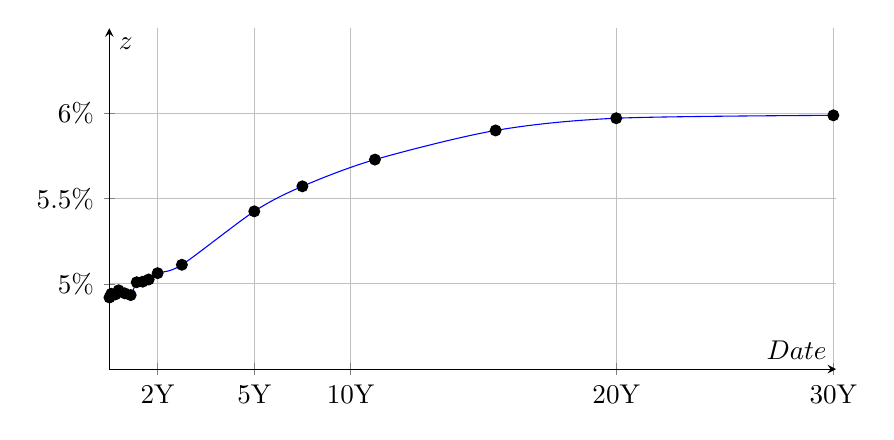
\begin{tikzpicture}[scale=.98]
		\begin{axis}[
			axis lines=middle,
			xlabel=$Date$,
			ylabel=$z$,
			xmin=0, xmax=11000,
			ymin=0.045, ymax=0.065,
			xtick={2, 731, 2194, 3650, 7672, 10958},
			ytick={0.045,0.05,0.055,0.06},
			xticklabels={Spot, 2Y, 5Y, 10Y, 20Y, 30Y},
			yticklabel={\pgfmathparse{100*\tick}\pgfmathprintnumber{\pgfmathresult}\%},
			width=11cm,
			height=6cm,
			grid=both,
			grid style={gray!50},
			scaled ticks=false %remove scientific notation
			]
		  
		  \addplot[only marks, mark=*] coordinates {
			(2, 0.049204)
			(30, 0.0494204)
			(50, 0.0493537)
			(91, 0.0493839)
			(141, 0.0496262)
			(232, 0.0494493)
			(323, 0.0493438)
			(414, 0.0500989)
			(505, 0.0501309)
			(596, 0.0502602)
			(731, 0.0506314)
			(1098, 0.0511228)
			(2194, 0.0542569)
			(2922, 0.0557244)
			(4020, 0.0572934)
			(5846, 0.0590024)
			(7672, 0.0597185)
			(10958, 0.0598892)
		  };
		  
		  \addplot[smooth,blue] coordinates {
			(2, 0.049204)
			(30, 0.0494204)
			(50, 0.0493537)
			(91, 0.0493839)
			(141, 0.0496262)
			(232, 0.0494493)
			(323, 0.0493438)
			(414, 0.0500989)
			(505, 0.0501309)
			(596, 0.0502602)
			(731, 0.0506314)
			(1098, 0.0511228)
			(2194, 0.0542569)
			(2922, 0.0557244)
			(4020, 0.0572934)
			(5846, 0.0590024)
			(7672, 0.0597185)
			(10958, 0.0598892)
		  };
		  \end{axis}
	  \end{tikzpicture}
	  \caption{Zero Rate for Different Maturities}
	\end{figure}
\end{frame}

\input{../../../LatexTemplatesAndSamples/last_slides_summary_and_questions.tex}

% \begin{frame}{Related Work and References}
% 	\begin{itemize}	
% 		\item Reference Lehman paper
% 		\item 1.9 Construction of Interest-rate Curves
% 	\end{itemize}
% \end{frame}

% \begin{frame}{Notes to add to other slides}
% 	\begin{itemize}
% 	  \item Look at web site of software company that writes very good articles but not such good software
% 	\end{itemize}
% \end{frame}

% \begin{frame}{Fixes for this Lecture}
% 	\begin{itemize}
% 		\item In swap section the flow vs coupon vs ntl exchange is confusing
% 		\item Change all cashflows to have negative first flow
% 		\item Add a slide with the dates and explain why there are zero rates
% 		\item Mention overlapping segments MM/FUT and also FUT/SWAP
% 		\item In our example we blend MM/FUT and use SWAP
% 		\item Should I show more than cents as my notional is just 100? Answer is yes but I need a footnote explaining why
% 		\item Add item about liquidity - Futures vs MM instrument with enough of amounts
% 		\item In the derivation put placeholders into tables that then derive when the slide animation shows the calculated values
% 	\end{itemize}
% \end{frame}

\end{document}
